%! Author = matteomagnini
%! Date = 05/03/25

%----------------------------------------------------------------------------------------
\chapter{Artificial intelligent systems}
\label{ch:intelligent-systems}

\begin{flushright}
\begin{minipage}{0.5\textwidth}
    What is \emph{intelligence}?

    What is \emph{\glsentrylong{AI}}?

    What are the characteristics of an \emph{intelligent system}?

    -- \textbf{\Cref{itm:rq0}}
\end{minipage}
\end{flushright}

\minitoc
%----------------------------------------------------------------------------------------


In this chapter, we introduce the concept of \emph{intelligence} providing one of the possible definition (\Cref{sec:what-is-intelligence}) starting from the sort of intelligence in animals and humans (\Cref{subsec:intelligence-in-nature}).
%
We then introduce intelligence in computer science with insights on reasoning, learning and agency (\Cref{subsec:intelligence-in-computer-science}).
%
Then, we focus on the core background of this thesis: \gls{AI} (\Cref{sec:ai}) by providing all the necessary notions the reader needs to understand the rest of the thesis.
%
Finally, we discuss the impact and implications of \gls{AI} in modern society (\Cref{sec:ai-and-society}).

%----------------------------------------------------------------------------------------
%-------------------------------------- Intelligence ------------------------------------
%----------------------------------------------------------------------------------------

\section{What is intelligence?}\label{sec:what-is-intelligence}

Intelligence is a concept that encompasses a wide range of abilities and characteristics of single \emph{individuals} or \emph{groups}.
%
From an \emph{evolutionary} perspective, intelligence characterises some animal species -- and organisms belonging to other biological kingdoms -- from simple forms of life.
%
In the history of our planet, carbon-based life evolved from unicellular organisms to multicellular organisms, and ultimately to complex organisms with specialized cells and tissues.
%
Some of these organisms (e.g., insects) developed skills -- such as \emph{navigation}, \emph{communication}, \emph{self-organisation}, \emph{adaptation}, and so on -- that \emph{are perceived} as intelligent abilities.
%
More evolved individuals (e.g., mammals) developed even more complex forms of intelligence, such as \emph{planning}, \emph{reasoning}, \emph{learning}, etc.


In much more recent history, the carbon-based life was not the only one to ``manifest'' intelligent behaviours.
%
With the invention of the computer, also machines can perform tasks that we consider intelligent.
%
To distinguish between the intelligence of living beings and that of machines, we refer to the former as \emph{natural intelligence} and to the latter as \emph{\gls{AI}}.


Intelligence originally emerged as a result of the evolutionary process and from the interaction of organisms with each others and their environment.
%
Later, we built machines that can perform tasks that require some sort of intelligent ability.
%
However, it is us -- as humans -- \emph{to attribute} the label of intelligent to someone or something and not to others.
%
Indeed, it is said that \emph{``intelligence is in the eye of the beholder''}.
%
In this sense, we can say that intelligence is not an absolute concept, but it should be considered under a relative perspective.


Giving a single rigorous definition of intelligence is not a trivial task.
%
Furthermore, there is not one single shape of intelligence, but it can be declined in many different ways (e.g., \emph{emotional intelligence}, \emph{social intelligence}, \emph{spatial intelligence}, etc.).
%
In this thesis we do not want to stay strictly dependant to a specific definition of intelligence, nevertheless it would be useful to provide a one.
%
We give a broad definition to help the reader to get more familiar with recurrent concepts that will appear later.
%
We choose to adopt a definition inspired by a notorious satirical essay by Cipolla~\cite{cipolla2013allegro}.
%
In \emph{``The basic laws of human stupidity''}, the author classifies \emph{individuals} into four categories based on the \emph{result} of their \emph{actions}:
%
\begin{itemize}
    \item \textbf{Stupid} $\rightarrow$ losses for others and for themselves;
    \item \textbf{Helpless} $\rightarrow$ benefits for others and losses for themselves;
    \item \textbf{Bandit} $\rightarrow$ losses for others and benefits for themselves;
    \item \textbf{Intelligent} $\rightarrow$ benefits for others and for themselves.
\end{itemize}
%
Now, what is a \emph{loss} or a \emph{benefit}?
%
We can see losses and benefits as the failure or success in -- fully or partially -- achieving a certain \emph{goal}.
%
With this respect we can state that:
%
\begin{definition}[Intelligence]
    \label{def:intelligence}
    an individual (or a group) has an intelligent behaviour if it is able to \textbf{perform actions} that lead to the \textbf{achievement} of a given \textbf{goal}.
\end{definition}
%
\Cref{def:intelligence} intentionally adopts a broad notion of intelligent behaviour.
%
Under this formulation, the ability to select actions that achieve a goal may also characterize simple reactive or feedback-based systems, as well as biological processes such as homeostasis.
%
For this reason, the definition should not be interpreted as a comprehensive or exclusive account of intelligence.
%
Rather, it serves as an operational definition, sufficient to delimit the class of systems considered in this work, namely artificial agents whose behaviour is guided by internal representations and decision mechanisms.


\Cref{def:intelligence} is also similar to the definitions of intelligence collected in the work of Legg and Hutter~\cite{DBLP:journals/mima/LeggH07}, such as the definition \emph{``The capacity to learn or to profit by experience''}~\cite{sternberg2000handbook}.
%
Broadly speaking, a common feature of these definitions is that intelligence is seen as a property of an individual \emph{interacting} with an external \emph{environment}, problem, or situation.
%
This interaction is fundamental to practically all proposed definitions of intelligence.
%
Another shared characteristic is the relationship between intelligence and the ability to succeed or \emph{profit} in achieving \emph{objectives}.
%
The notion of success or profit implies the existence of a specific \emph{goal}, although the exact nature of the goal may vary across individuals or contexts.
%
What matters is the capacity of the individual to carefully select actions that lead to the accomplishment of these goals.
%
The greater this capacity to succeed across a variety of goals, the greater the individual's intelligence.
%
This perspective aligns with the idea that intelligence is not a fixed attribute but rather a dynamic ability to adapt and perform effectively in diverse scenarios.


\subsection{Natural intelligence}\label{subsec:intelligence-in-nature}

In order to survive in their environment, animals -- but also other organisms of different kingdoms such as plants or fungi -- have developed a set of abilities and some of them are perceived as intelligent.
%
For the sake of simplicity, we will consider just to animals, but many of the concepts we will talk about can be extended to other organisms.
%
Animals have a \emph{body}, and they are \emph{situated} in the physical world.
%
Through sensory organs, they can \emph{perceive} the environment and with muscles they can \emph{interact} with it.
%
They are \emph{autonomous} individuals, i.e., they are able to perform actions without the need of an external controller.


All animals are able to keep themselves alive (\emph{self-sufficiency}) until natural death or an accident occurs.
%
In addition to self-sufficiency, animals contribute to the survival of their species generating offspring.
%
To do so, they need to navigate the environment, find food, avoid predators, reproduce, and so on.


Humans have developed two main characteristics about intelligence that are no match for any other animals: \emph{reasoning} and \emph{learning}.
%
\paragraph{Reasoning}
%
Logical reasoning, or simply reasoning, is a process of drawing conclusions from premises.
%
There exists three main ways of reasoning:
%
\begin{itemize}
    %
    \item \textbf{Deductive reasoning} $\rightarrow$ it is a top-down approach that starts from a general statement and derives specific conclusions.
    %
    For example, if we know that \emph{all humans are mortal} and \emph{Socrates is a human}, we can conclude that \emph{Socrates is mortal}.
    %
    Deductive reasoning can be compared to what Kahneman calls \emph{System 2} in his book \emph{Thinking, Fast and Slow}~\cite{kahneman2011thinking}.
    %
    Kahneman describes the second system as \emph{slow thinking}, which is deliberate, effortful, logical and more rational.
    %
    \item \textbf{Inductive reasoning} $\rightarrow$ it is a bottom-up approach that starts from specific observations and derives general conclusions.
    %
    For example, if we observe that \emph{the sun rises every day}, we can conclude that \emph{the sun will rise tomorrow}.
    %
    Inductive reasoning can be mapped in the \emph{System 1} -- i.e., \emph{fast thinking} -- of Kahneman, which is automatic, effortless, intuitive and emotional.
    %
    However, this mapping should be interpreted as partial: while some forms of inductive reasoning may rely on rapid, intuitive mechanisms, \emph{System 1} also includes innate or pre-attentive processes that are not the result of learning, and more complex inductive inferences may involve deliberative components typically associated with \emph{System 2}.
    %
    \item \textbf{Abductive reasoning} $\rightarrow$ it is a form of reasoning that starts from an observation and seeks the simplest and most likely explanation (i.e., \emph{Occam's razor}).
    %
    For example, if we observe that \emph{the grass is wet}, we can conclude that \emph{it rained last night}.
    %
    This kind of reasoning is the same that is adopted by detectives to solve crimes.
    %
    Abduction also requires the use of statistics and probabilities, and therefore it deals with uncertainty (\emph{``Once you eliminate the impossible, whatever remains, no matter how improbable, must be the truth''---Arthur Conan Doyle}\footnote{a person must be aware of all the possibilities in order to not fall into a deductive error.}).
\end{itemize}


\paragraph{Learning}
%
Human beings can perform a vast array of tasks, and their ability to learn new ones is a cornerstone of their intelligence.
%
Learning is a process that allows individuals to \emph{model reality}, adapt to their environment, and share knowledge with others.
%
Broadly speaking, humans acquire new skills and knowledge in two primary ways: by generalising experience -- e.g., via \emph{inductive} reasoning --, or by \emph{deductively} inferring new knowledge from what they already hold or can obtain from others---e.g., through direct communication (talking) or indirect communication (reading)~\cite{human-reasoning-1994}.
%
In the former case, novel knowledge is formed in the learner's mind by interacting with the environment and interpreting sensory input.
%
In the latter case, knowledge is represented symbolically (e.g., through words, gestures, or diagrams), enabling communication and the transfer of meaning between individuals.
%
This symbolic representation is crucial for sharing complex ideas and building upon the collective knowledge of a society.

Animals, too, exhibit learning abilities, though the mechanisms and extent vary widely across species.
%
For instance, many animals rely on experience to adapt to their environment, such as learning to navigate, find food, or avoid predators.
%
Some species, like primates and certain birds, demonstrate the ability to use symbols or tools, which suggests a rudimentary form of modeling reality and reasoning about their surroundings~\cite{shettleworth2010cognition}.
%
In both humans and animals, learning is deeply tied to the interaction with the environment, where experiences shape the internal models of reality that guide future actions.

In humans, the ability to reason about acquired knowledge is particularly advanced.
%
This reasoning allows individuals to not only apply learned concepts but also to refine and expand them, often by integrating new information with existing symbolic representations.
%
Such reasoning processes are essential for problem-solving, planning, and innovation, which are hallmarks of human intelligence~\cite{DBLP:journals/mima/LeggH07}.
%
Moreover, the ability to share knowledge through symbolic means, such as language, has enabled humans to build complex societies and advance technologically.


\subsection{Intelligence in computer science}
\label{subsec:intelligence-in-computer-science}
%
Since the automation of computation with the invention of the computer, intelligence has always been a central topic in computer science.
%
Officially, the field of \gls{AI} was born in 1956 at the Dartmouth Conference, where a group of researchers gathered to discuss the possibility of \emph{computing towards intelligence}.
%
In this section, we provide a high-level introduction of how machines can mimic the processes of reasoning and learning that we find in natural intelligence.
%
Later, in \Cref{sec:ai} we give a detailed background on \gls{AI}.


\subsubsection{Reasoning}\label{subsubsec:reasoning-cs}
%
Every form of reasoning presupposes a structured connection between \emph{reality} and its \emph{representation}.
%
In symbolic approaches to \gls{KR}, this connection is mediated through \emph{symbols}, where the interplay between \emph{signifier} and \emph{signified} enables the encoding of meaning.
%
Symbols thus act as the bridge between the external world and computational processes, allowing reasoning systems to manipulate abstract entities while still preserving a link to the underlying semantics of the domain.
%
In this sense, reasoning is not only the mechanical application of rules, but also the interpretative activity that derives new knowledge by operating on representations whose significance is grounded in the symbolic layer of \gls{KR}.


Symbolic \gls{KR} has always been regarded as a key issue since the early days of \gls{AI}, under the assumption that intelligent behavior requires explicit forms of knowledge and mechanisms to represent and manipulate it~\cite{DBLP:journals/cacm/NewellS76,BRACHMAN2004327}.
%
When compared to arrays of numbers, symbolic \gls{KR} is far more flexible and expressive, and, in particular, more intelligible---both machine- and human-interpretable.
%
Historically, most \gls{KR} formalisms and technologies have been designed on top of \emph{computational logic}~\cite{lloyd1990computational}, that is, the exploitation of formal logic in computer science.
%
Consider, for instance, \emph{deductive databases}~\cite{green1968}, \emph{description logics}~\cite{DBLP:conf/dlog/2003handbook}, \emph{ontologies}~\cite{cimiano2006-ontologies}, \emph{Horn} logic~\cite{Mcnulty1977}, \emph{higher-order} logic~\cite{VanBenthem2001}.


Reasoning in computer science involves the process of deriving conclusions from a set of premises or facts, often encoded in a formal language.
%
Logic reasoners, such as Prolog-based systems like tuProlog~\cite{DBLP:conf/padl/DentiOR01}, play a central role in automating this process.
%
These reasoners typically follow a sequence of steps:
%
\begin{itemize}
    \item \textbf{Parsing}, the reasoner first parses the input knowledge base, which consists of facts, rules, and queries, into an internal representation;
    %
    \item \textbf{Inference}, using inference rules, such as \emph{modus ponens}~\cite{DBLP:books/daglib/0076838}, the reasoner derives new facts or verifies the truth of a query.
    %
    \item \textbf{Unification}, a key operation in logic reasoning is unification, where variables in predicates are matched with constants or other variables to satisfy logical constraints;
    %
    \item \textbf{Search}: the reasoner explores the search space of possible solutions, often using strategies like depth-first search or breadth-first search, depending on the implementation;
    %
    \item \textbf{Result generation}, finally, the reasoner provides the results of the reasoning process, which could be a solution to the query, a proof, or a set of derived facts.
\end{itemize}
%
For example, in a Prolog-based system, a query is resolved by attempting to unify it with facts or the heads of rules in the knowledge base, recursively applying the rules' bodies until a solution is found or all possibilities are exhausted.
%
Logic reasoners are widely used in various applications, including expert systems, semantic web technologies, and automated theorem proving, due to their ability to handle complex symbolic reasoning tasks efficiently.



\subsubsection{Learning}\label{subsubsec:machine-learning-cs}
%
The learning process performed by machines is called \glsfull{ML}.
%
\gls{ML} is a wide umbrella term that encompasses a variety of different ways of learning and different learning tasks.
%
A widely adopted definition of \gls{ML} is the one given by Tom Mitchell in 1997~\cite{DBLP:books/daglib/0087929}:
%
\begin{definition}[Machine Learning]
    \label{def:ml}
    a computer program is said to learn from experience $E$ with respect to some class of tasks $T$ and performance measure $P$ if its performance at tasks in $T$, as measured by $P$, improves with experience $E$.
\end{definition}
%
The software component deputed to learning is referred as \emph{model}, \emph{learner} or \emph{predictor} (and possibly other names).
%
The experience $E$ can be represented as a given dataset, i.e., a collection of input data, but there could be other ways (e.g., through \gls{RL}).
%
The input can come in different shapes, e.g., \emph{tabular data}, \emph{images}, \emph{text}, etc.
%
Each input type is represented in different ways to be interpreted by a machine: an entry in a table is represented as a vector of features, an image is usually represented as a matrix, or a tensor, and a text can be represented as a vector of word embeddings.
%
There can be a variety of different tasks $T$ and performance measures $P$.
%
In the rest of this section, we will provide a brief overview of the most common tasks and performance measures.


The most common macro \gls{ML} tasks are:
%
\begin{itemize}
    \item \textbf{Classification} $\rightarrow$ given the input data $X={x_1, x_2, \dots, x_n}$, the task is to predict a label $y$ (a.k.a., output) from a finite set of labels $Y=\{y_1, y_2, \dots, y_m\}$.
    %
    The input is made of numerical features $x_i$ that can either be binary, categorical, or continuous.
    %
    Ultimately, the goal is to learn a prediction function $\pi^{*}: X \rightarrow Y$;
    %
    \item \textbf{Regression} $\rightarrow$ the task consists in predicting a continuous value $y$ from the input data $X$.
    %
    Similarly to classification, the goal is to learn the optimal predictor that maps the input $X$ to the output $Y$ (usually $Y=\mathbb{R}$);
    %
    \item \textbf{Clustering} $\rightarrow$ the task is to group the input data $X$ into $k$ clusters according to some strategy (e.g., usually a distance function).
    %
    A cluster is a subset of the input data $X$ that is \emph{similar to each other} and \emph{dissimilar from the data in other clusters}.
    %
    Clustering predictors can be considered as classifiers upon anonymous classes.
    %
\end{itemize}
%
To approximate $\pi^{*}$, a learning algorithm is used.
%
Depending on the type of learning algorithm, the learning process can be \emph{supervised}, \emph{unsupervised}, or \emph{reinforcement}.
%

\paragraph{Supervised}
%
A \gls{ML} process is \emph{supervised} if it is trained on a labelled dataset, where each data point is associated with a corresponding label that represents the desired output.
%
The training set is made of pairs $(x_i, y_i)$, where $x_i$ is the input data and $y_i$ is the corresponding label.
%
The goal of the learning process is to learn a function $f$ that maps the input data $x_i$ to the corresponding label $y_i$, such that $f(x_i) \approx y_i$ for almost all training examples~\footnote{the learning process can sacrifice accuracy on some training examples to improve generalization on unseen data.}.
%
The function $f$ is usually a mathematical model that is trained on the training set by minimizing a loss function, which quantifies the error between the predicted output $\hat{y}_i = f(x_i)$ and the true label $y_i$.
%
For example, in a binary classification task, the loss function could be the binary cross-entropy, while in a regression task, it could be the mean squared error.
%
Once trained, the model can generalize to unseen data, predicting labels for new inputs based on the patterns it has learned from the training set.
%
An example of supervised learning is email spam detection, where the input $x_i$ could be the content of an email, and the label $y_i$ could be either \emph{spam} or \emph{not spam}.
%
The model learns to classify emails by analyzing a dataset of labelled examples and can then predict whether a new email is spam or not.
%

\paragraph{Unsupervised}
%
In unsupervised learning, the learning task consists of discovering patterns, structures, or relationships within a dataset without relying on labeled outputs.
%
The goal is to find an optimal representation or grouping of the data based on an objective criterion, such as minimizing intra-cluster distances or maximizing data variance.
%
Common tasks in unsupervised learning include \emph{clustering}, where data points are grouped into clusters based on similarity, and \emph{dimensionality reduction}, where the data is transformed into a lower-dimensional space while preserving its essential structure.
%
For example, in clustering, the \emph{k-means} algorithm partitions a dataset into \(k\) clusters by iteratively assigning data points to the nearest cluster centroid and updating the centroids to minimize the total intra-cluster variance~\cite{lloyd1982least}.
%
Another example is \gls{PCA}, a dimensionality reduction technique that identifies the directions (principal components) in which the data varies the most, enabling efficient data compression and visualization~\cite{pearson1901lines}.


\paragraph{\Glsentrylong{RL}}
%
In reinforcement learning, the learning task consists of letting an agent estimate \emph{optimal plans or policies} by interacting with an environment and receiving feedback in the form of rewards or penalties.
%
The agent's goal is to maximize the cumulative reward over time by learning which actions to take in different states of the environment.
%
This process is typically modeled as a \gls{MDP}, which is defined by a set of states, a set of actions, a transition function that describes the probabilities of moving between states, and a reward function that assigns a numerical value to each state-action pair~\cite{DBLP:books/lib/SuttonB98}.
%
For example, consider a ground robot that performs phototaxis, i.e., it moves towards a light source.
%
The robot can perceive its environment through sensors that detect the light intensity and can perform actions such as moving forward, turning left, or turning right.
%
When the robot moves closer to the light source, it receives a positive reward, while moving away results in a negative reward.
%
Over time, the robot learns a policy that maps states to actions, allowing it to navigate effectively towards the light source by maximizing its cumulative reward.

%
%\subsubsection{Agents}\label{subsubsec:agents}
%%
%We will use the term software \emph{agent} (just \emph{agent} for simplicity) from now on to refer to a software process that has particular characteristics.
%%
%One of these is \emph{autonomy}.
%%
%Autonomy is the ability of an agent to act without the direct control of humans or other agents.
%%
%Technically speaking, an agent encapsulates its own thread of control.
%%
%Autonomy is not absolute, but it is a matter of degree; e.g., self-sufficiency increases the degree of autonomy of an agent.
%%
%Autonomy -- \emph{per se} -- does not imply intelligence.
%%
%For example, from a biological perspective, a cell has some degree of autonomy (e.g., it has boundaries, it interacts with the environment, etc.), but certainly we do not consider it an intelligent entity.
%%
%However, it is a fundamental trait of living systems and life evolved towards more and more autonomous systems.
%
%
%A \emph{robot} -- i.e., an \emph{embodied agent} -- that is able to recognise when its battery is low and to recharge itself is more autonomous than a robot that needs to be recharged by a human.




%----------------------------------------------------------------------------------------
%---------------------------------------- AI --------------------------------------------
%----------------------------------------------------------------------------------------

\section[Artificial Intelligence]{\Glsentrylong{AI}}
\label{sec:ai}

The wide range of \gls{AI} techniques are divided into many categories, including two major ones: \emph{symbolic} and \emph{sub-symbolic} \gls{AI}.
%
\Cref{fig:ai-map} provides an overview of \gls{AI} fields, highlighting the distinction between symbolic and sub-symbolic approaches.
%
The thing that distinguishes these two categories is the way they \emph{represent knowledge} and how they process it.
%
No intelligence can exist without knowledge and no computation can occur in lack of representation.
%
In the rest of the thesis, we will use the term symbolic (resp., sub-symbolic) \gls{AI} and symbolic (resp., sub-symbolic) \gls{KR} almost interchangeably.
%
Symbolic \gls{AI} is based on \emph{symbols}, which come with a \emph{meaning} and could be manipulated according to the formalism and rules of a given \gls{AI} system.
%
On the other hand, sub-symbolic \gls{AI} is based on a numerical representation -- a.k.a., sub-symbolic -- where the numbers are not directly interpretable.
%
Numbers are technically symbols, but numbers, arrays and their functions are not recognised as means for symbolic \gls{KR}.
%
According to Van Gelder~\cite{DBLP:conf/ogai/Gelder90}, in order to be considered symbolic, \gls{KR} approaches must:
%
\begin{requirements}
    %
    \item \label{itm:symbolic-req-1} involve a set of symbols;
    %
    \item \label{itm:symbolic-req-2} the symbols can be combined following a set of grammatical rules;
    %
    \item \label{itm:symbolic-req-3} elementary symbols and combinations of symbols can be assigned a meaning.
    %
\end{requirements}
%
\begin{figure}
    \centering
    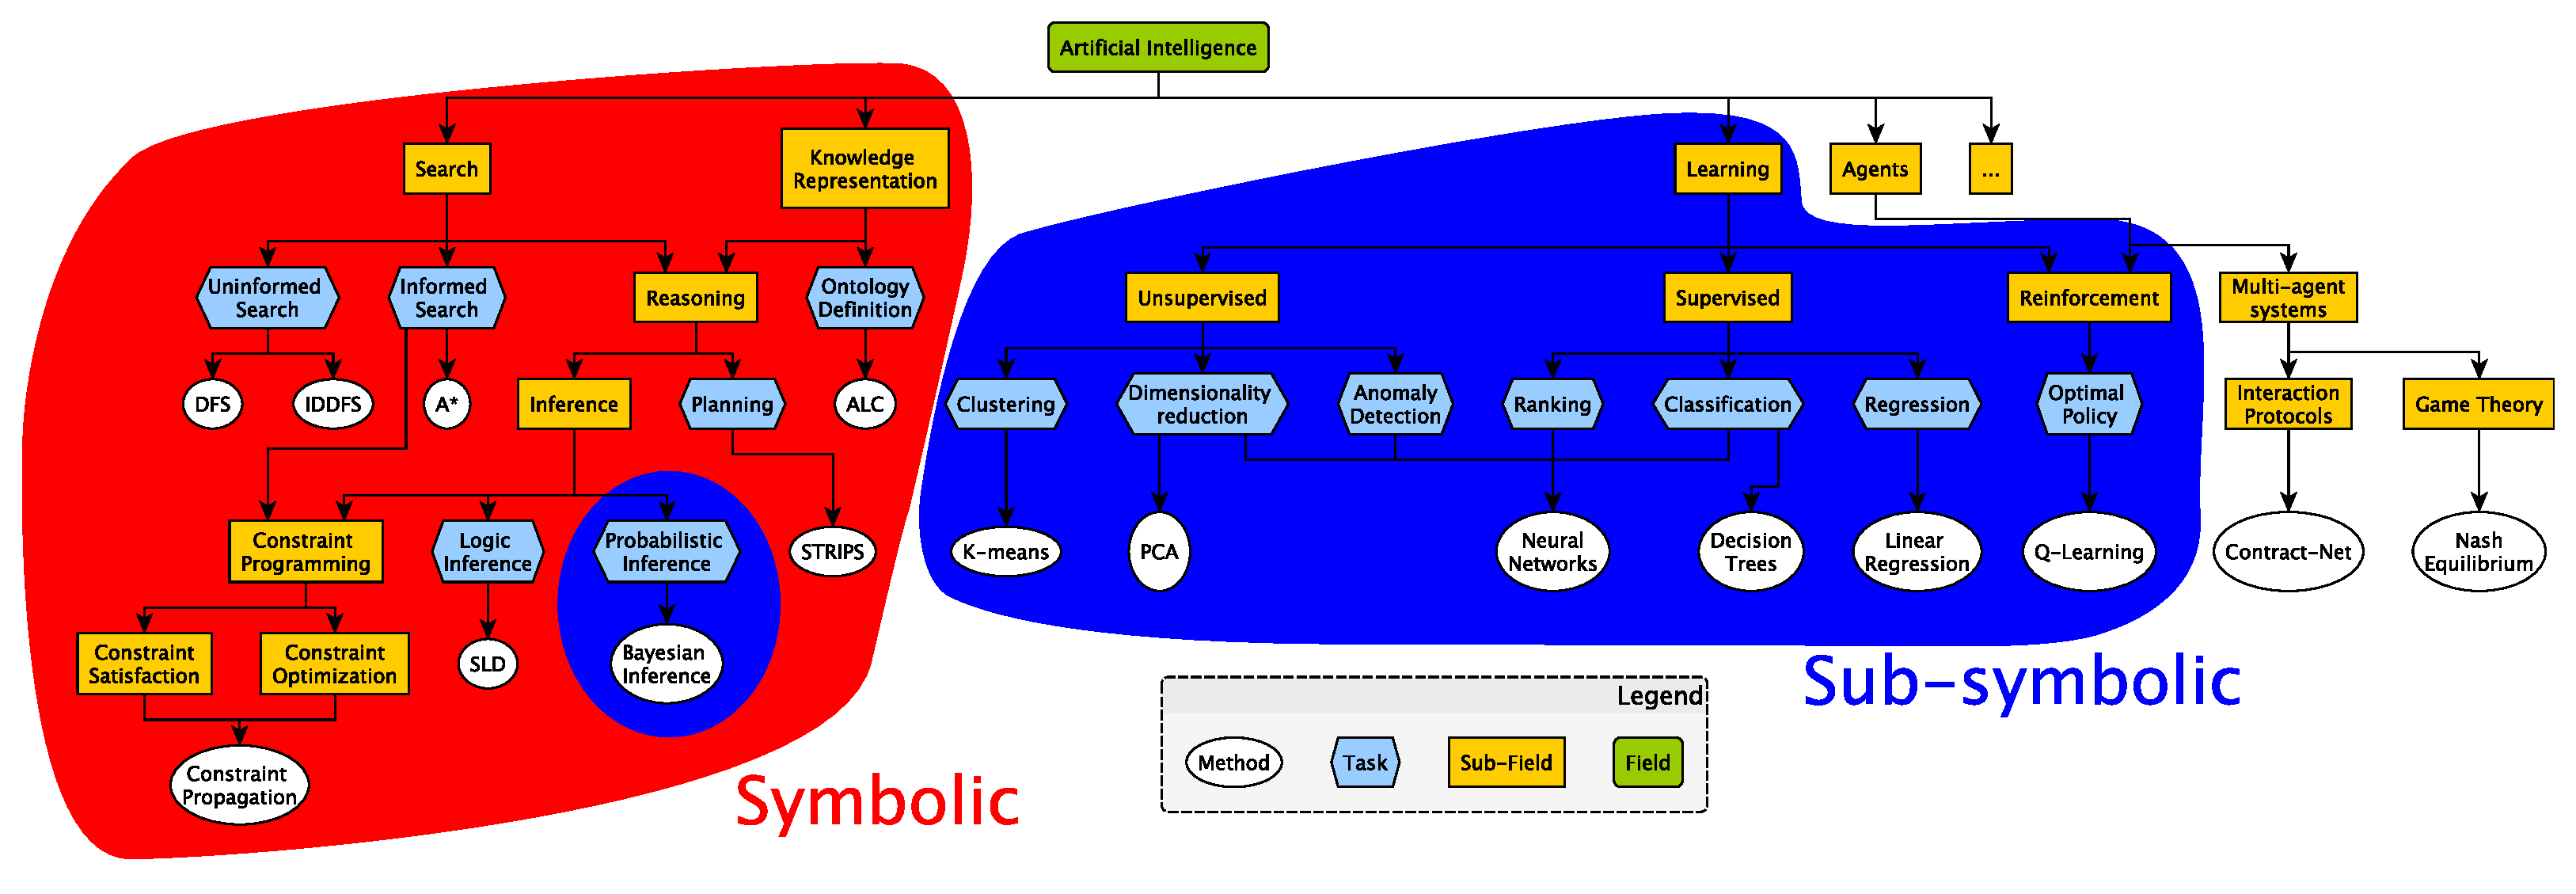
\includegraphics[width=\textwidth]{figures/ai-map2}
    \caption[Overview of the field of artificial intelligence]{
        \Gls{AI} map (not exhaustive) illustrating the main subfields with a focus on symbolic and sub-symbolic approaches.
        %
        On the left side, symbolic \gls{AI} is represented by search algorithms, \glspl{KR}, and reasoning.
        %
        On the right side, sub-symbolic \gls{AI} is represented by learning technique families, such as unsupervised learning, supervised learning, and reinforcement learning.
        %
        The figure is a simplified representation to give the reader a general idea of the landscape of \gls{AI}.
        %
        Notably, learning-based approaches are not necessarily subsymbolic.
        %
        For instance, \gls{ILP} and \glsentryshort{DT} learning induce explicit symbolic structures whose components retain a well-defined and compositional semantics, despite being learned from data.
    }
    \label{fig:ai-map}
\end{figure}


\paragraph{Local vs. distributed}
%
Multidimensional arrays are the fundamental building block of sub-symbolic data representation.
%
Formally, a $D$-order array is an ordered container of real numbers, where $D$ indicates the number of indices required to access each element.
%
We refer to 1-order arrays as \emph{vectors}, 2-order arrays as \emph{matrices}, and arrays of order greater than two as \emph{tensors}.
%
In sub-symbolic tasks based on arrays, information is typically conveyed both by the values stored in the array and their position within it.
%
The dimensions of the array -- denoted as $(d_1 \times \dots \times d_D)$ -- also play a crucial role, as sub-symbolic systems are usually designed to operate on arrays of fixed shape.
%
That is, the values of $d_1, \dots, d_D$ are chosen at design time and remain unchanged thereafter.
%
This violates \Cref{itm:symbolic-req-2} above; accordingly, we define sub-symbolic \gls{KR} as the task of encoding information into rigid numeric arrays.
%
\emph{Local} and \emph{distributed} representations are two key modes for encoding data into such arrays.
%
In local representations, each entry in the array corresponds to a well-defined concept from the target domain---its semantic meaning is clear and independent.
%
In distributed representations, by contrast, individual values carry little or no standalone meaning: their interpretation depends on the configuration of values across a neighbourhood in the indexing space.
%
Consequently, while the exact location of values is largely irrelevant in local representations, it becomes essential in distributed ones.
%
Notably, distributed representations violate \Cref{itm:symbolic-req-3}, and for this reason, recent literature often labels as \emph{sub-symbolic} those predictors that rely on distributed encoding of data.

%----------------------------------------------------------------------------------------
%------------------------------------ Symbolic AI ---------------------------------------
%----------------------------------------------------------------------------------------

\subsection[Symbolic AI]{Symbolic \Gls{AI}}\label{subsec:symbolic-ai}
%
Symbolic \gls{AI} has been regarded as crucial since \gls{AI}'s inception.
%
Symbolic \gls{KR} offers enhanced flexibility, expressiveness, and intelligibility, being interpretable both by machines and by humans.

\paragraph{Intentional vs. extensional}
%
In formal logic, one may define concepts either \emph{extensionally} or \emph{intensionally}.
%
Extensional definitions are direct representations of data.
%
For example, the set of square numbers admits the extensional definition $\{0,1,4,9,16,\dots\}$ by listing every member explicitly.
%
Conversely, an \emph{intensional} definition is an indirect representation of data.
%
In \gls{FOL}, this corresponds to defining a relation via a formula; for instance, the set of square numbers can be defined as $\{\,x\mid \exists n\in\mathbb{Z}\,(x = n^2)\}$ which succinctly encodes an infinite extension with a single schema.
%
Recursive intensional predicates further enhance expressivity: for example, the ancestor relation can be axiomatized by $\mathit{Ancestor}(x,y)\;\Leftrightarrow\;\mathit{Parent}(x,y)\;\lor\;\exists z\,[\,\mathit{Parent}(x,z)\wedge\mathit{Ancestor}(z,y)\,]$ allowing a compact representation of an infinite set of pairs with a finite rule.
%
In formal logic, intensional definitions are prized for their ability to model potentially unbounded domains within finite logical formalisms.


\paragraph{Expressiveness vs. tractability}
%
\begin{SCfigure}
    \centering
    \includegraphics[width=0.58\textwidth]{figures/venn_diagram_logics}
    \caption[Venn diagram of different logic families]{
        %
        Venn diagram of different logic families, illustrating the trade-off between expressiveness and tractability.
        %
        \Gls{FOL} is the most expressive logic -- not the most expressive logic in general -- encompassing all others.
        %
        On the other hand, propositional logic is the least expressive, as it can only represent atomic propositions and their combinations.
        %
        All the other logics fall somewhere in between, with varying degrees of expressiveness and tractability.
    }
    \label{fig:venn-diagram-logics}
\end{SCfigure}

%
Tractability addresses the theoretical question of whether a logic reasoner can determine the truth of a given formula within feasible time and space bounds.
%
The answer is deeply tied to the specific reasoning algorithm and the logic's formal properties.
%
Depending on the features a logic provides -- such as quantifiers, function symbols, or recursive definitions -- it may be more or less expressive.
%
The higher the expressiveness, the more complex the problems that can be represented and reasoned about, but this also increases the computational burden.
%
This well-known phenomenon is often referred to as the expressiveness/tractability trade-off~\cite{DBLP:journals/jlp/CadoliS93,BRACHMAN2004327,DBLP:journals/ci/LevesqueB87}.
%
In practice, highly expressive logics make it easier for human users to model rich domains, often requiring fewer and more concise formulas.
%
However, this comes at the cost of automated inference, which may become computationally intractable, undecidable, or non-terminating in the general case.
%
To mitigate this issue, various fragments and extensions of \gls{FOL} have been identified, each providing different tradeoffs between what can be expressed and what can be decided efficiently.
%
\Cref{fig:venn-diagram-logics} illustrates the relationships among different logic families, highlighting the trade-off between expressiveness and tractability.


\subsubsection[First-order logic]{\Glsentrylong{FOL}}\label{subsubsec:first-order-logic}
%
\Gls{FOL} is a general-purpose formalism that underpins most symbolic \gls{KR} systems.
%
It enables both human and computational agents to model entities and their interrelations through predicates and terms within a defined domain of discourse.
%
Its syntax comprises variables (quantified explicitly or implicitly), constants, function symbols, and predicate symbols, which are combined via logical operators such as conjunction (\(\wedge\)), disjunction (\(\vee\)), implication (\(\rightarrow\)), and equivalence (\(\leftrightarrow\)).
%
\Gls{FOL} allows for both \emph{extensional} and \emph{intensional} definitions.
%
Recursive intensional definitions, in particular, are powerful, enabling finite representations of infinite sets.
%
Despite its flexibility, \gls{FOL} is semi-decidable in general: there is no algorithm that can determine the truth of every \gls{FOL} formula in finite time, which limits its use in systems requiring guaranteed termination~\cite{DBLP:conf/dlog/2003handbook}.


\subsubsection{Horn logic}\label{subsubsec:horn-logic}
%
Horn logic is a significant subset of \gls{FOL}, offering a balanced trade-off between theoretical expressiveness and practical tractability~\cite{DBLP:journals/jcss/Makowsky87}.
%
It is built around the concept of \emph{Horn clauses}~\cite{DBLP:journals/jsyml/Horn51}, which are formulas in \gls{FOL} that exclude quantifiers and consist of a disjunction of predicates, with at most one non-negated literal.
%
Alternatively, a Horn clause can be expressed as an implication where the consequent is a single predicate and the antecedent is a conjunction of predicates: \(h \gets b_1, \dots, b_n\).
%
Here, \(\gets\) denotes logical implication (from right to left), commas represent logical conjunctions, and \(b_i\) as well as \(h\) are predicates of arbitrary arity, potentially containing \gls{FOL} terms such as variables, constants, or functions.

Horn clauses can be interpreted as \emph{if-then} rules written in reverse order, where only conjunctions of predicates are allowed in the antecedent.
%
In essence, Horn logic is a constrained subset of \gls{FOL} characterized by the following limitations:
%
\begin{inlinelist}
%
    \item formulas are reduced to clauses, containing only predicates, conjunctions, and a single implication operator;
    %
    \item operators such as \(\lor\), \(\leftrightarrow\), or \(\neg\) (negation) are not allowed;
    %
    \item variables are implicitly quantified; and
    %
    \item terms behave as they do in \gls{FOL}.
    %
\end{inlinelist}


\subsubsection{Datalog}\label{subsubsec:datalog}
%
Datalog is a declarative query language and a restricted subset of \gls{FOL}, designed for deductive databases and knowledge representation~\cite{DBLP:journals/jcss/AjtaiG94}.
%
It represents knowledge using function-free Horn clauses, as defined in \Cref{subsubsec:horn-logic}.
%
This restriction eliminates the use of function symbols, thereby forbidding structured terms such as recursive data structures.
%
As a result, Datalog is well-suited for applications requiring finite and decidable reasoning, as the absence of function symbols ensures termination of inference algorithms.
%
Similar to Horn logic, Datalog's knowledge bases consist of sets of function-free Horn clauses, which are interpreted as rules and facts.
%
Rules in Datalog follow the form \(h \gets b_1, \dots, b_n\), where \(h\) is the head of the rule and \(b_1, \dots, b_n\) are the body predicates.
%
Unlike general \gls{FOL}, Datalog does not allow disjunctions, negations, or explicit quantifiers, as variables are implicitly universally quantified.
%
Datalog is widely used in areas such as \glspl{KG}, semantic web technologies, and database systems, where efficient reasoning over large datasets is required.
%
Its simplicity and computational efficiency make it a practical choice for symbolic \gls{AI} tasks that demand tractable reasoning.


\subsubsection[Description logic]{\Glsentrylong{DL}}\label{subsubsec:dl}
%
\Gls{DL} are a family of subsets of \gls{FOL}, typically involving limited or no quantifiers, no structured terms, and no \textit{n}-ary predicates where \(n \geq 3\)~\cite{DBLP:books/daglib/0041477}.
%
In essence, \gls{DL} represents knowledge using constants and variables, along with atomic, unary, and binary predicates.


The differences among specific variants of \gls{DL} lie in the set of supported logical connectives and whether negation is allowed.
%
The wide variety of \gls{DL} stems from the well-known trade-off between expressiveness and tractability.
%
Depending on the application, one may prefer a more expressive \gls{DL} variant, which offers richer features at the cost of reduced tractability or even decidability of algorithms manipulating the knowledge, or vice versa.


In \gls{DL}, it is common practice to use specific terminology for different elements of knowledge representation:
%
\begin{itemize}
    %
    \item Constant terms are referred to as \textit{individuals}, as each constant represents a single entity within a domain.
    %
    \item Unary predicates are called \textit{classes} or \textit{concepts}, grouping sets of individuals for which the predicate holds true.
    %
    \item Binary predicates are referred to as \textit{properties} or \textit{roles}, connecting pairs of individuals.
    %
\end{itemize}
%

Using this nomenclature, knowledge in \gls{DL} can be represented by associating entities with constants (e.g., URLs) and defining concepts and properties accordingly.
%
Binary predicates are particularly significant as they enable the connection of pairs of entities.
%
This is typically achieved through subject-predicate-object triplets, represented as ground binary predicates of the form \(\langle a \, f \, b\rangle\) or \(f(a, b)\), where \(a\) is the subject, \(f\) is the predicate, and \(b\) is the object.

Collections of such triplets form \glspl{KG}, which are directed graphs where vertices represent individuals and arcs represent binary properties connecting these individuals.
%
\glspl{KG} may explicitly or implicitly instantiate a specific ontology, which is a formal description of classes characterizing a domain, their relationships (e.g., inclusion, exclusion, intersection, equivalence), and the properties they must or must not include.


\glspl{DL} are widely used in applications such as semantic web~\cite{DBLP:conf/coopis/GangemiM03} and ontology engineering~\cite{DBLP:books/ios/HGJKP2016}, where efficient reasoning and knowledge representation are essential.
%
Their ability to balance expressiveness and computational efficiency makes them a cornerstone of symbolic reasoning systems.


\subsubsection[Ontologies and knowledge graph]{Ontologies and \glsentrylong{KG}}\label{subsubsec:ontologies-and-kg}
%
An ontology is a formal and explicit specification of a shared conceptualisation of a domain~\cite{DBLP:books/daglib/p/Grimm10}.
%
It provides a structured vocabulary to describe the entities relevant in that domain, along with their attributes and the relationships among them.
%
This organisation enables both human understanding and machine-based reasoning.

Ontologies are typically expressed using \glspl{DL}, a family of logic-based formalisms for knowledge representation.
%
\Glspl{DL} define three main components:
%
\begin{inlinelist}
    %
    \item\emph{concepts} (or \emph{classes}), which group entities sharing similar features;
    %
    \item\emph{individuals} (or \emph{instances}), which are the concrete elements of the domain;
    %
    \item\emph{roles} (or \emph{properties}), which describe binary relationships between individuals.
    %
\end{inlinelist}
%
Different \glspl{DL} vary in their expressive power: for example, \gls{EL} supports only conjunction and existential quantification to ensure efficient reasoning, while more expressive DLs like \gls{ALC} allow for full Boolean operators and universal quantification.

Concepts are typically denoted using capital italic letters, such as $\mathit{Animal}$ or $\mathit{Cat}$.
%
These can be combined using logical constructors like intersection ($\sqcap$), union ($\sqcup$), or negation ($\lnot$) to form more complex classes.
%
A statement like $\mathit{Cat} \sqsubseteq \mathit{Animal}$ expresses that all cats are animals.

Individuals are constants representing specific entities in the domain and are usually written in monospaced lowercase, for example \texttt{tom}.
%
Membership of an individual in a concept is denoted using the ``is-a'' relation, written as \texttt{tom}~:~$\mathit{Cat}$, meaning ``Tom is a cat.''
%
Each individual may belong to multiple concepts.

Roles represent binary relations between individuals and are written in lowercase sans-serif font, such as \textsf{eats}.
%
They connect pairs of individuals, and their domain and range can be restricted using expressions such as $\textsf{eats} \sqsubseteq \mathit{Animal} \times \mathit{Edible}$.
%
Assertions like $\textsf{eats}(\texttt{tom}, \texttt{mouse})$ state that Tom eats the mouse.

The subsumption relation ($\sqsubseteq$) is used to express inclusion between concepts or roles.
%
For instance, $\mathit{Cat} \sqsubseteq \mathit{Animal}$ means that every cat is also an animal, and $\textsf{predatorOf} \sqsubseteq \textsf{eats}$ means that every predator-prey relationship implies eating.
%
Special concepts such as $\top$ and $\bot$ are used to denote the most general and the most specific concepts, respectively.

Collections of such axioms form an ontology.
%
\Gls{TBOX} define concepts and roles and their interrelations, while \gls{ABOX} specify which individuals belong to which concepts or are related via which roles.

\Glspl{KG} also provide a structured way to represent knowledge as graphs.
%
They consist of triplets (or \emph{facts}) of the form $(s, p, o)$, where $s$ is the subject, $p$ is the predicate (or property), and $o$ is the object.
%
These triplets form a directed graph where nodes represent individuals and edges represent relationships.

Unlike ontologies, KGs do not necessarily impose formal constraints on the structure or semantics of the triplets.
%
This flexibility allows for representing heterogeneous and incomplete data.
%
However, some \glspl{KG} are explicitly grounded in an ontology, and may follow its vocabulary and logical constraints.

In summary, ontologies and knowledge graphs both aim to formally capture structured knowledge.
%
Ontologies provide formal semantics and enable logical reasoning, while knowledge graphs emphasise scalability and flexibility in representing factual data.


\subsubsection{Propositional Logic}\label{subsubsec:propositional-logic}
%
Propositional logic is a restricted subset of \gls{FOL} in which quantifiers, terms, and non-atomic predicates are absent.
%
Its language consists solely of atomic propositions -- also called 0-ary predicates -- combined using standard logical connectives such as conjunction ($\land$), disjunction ($\lor$), negation ($\lnot$), and implication ($\rightarrow$).
%
Each proposition can be interpreted as a Boolean variable that takes a truth value in \{\texttt{true}, \texttt{false}\}.
%
The semantics of propositional logic aligns with Boolean algebra, making it straightforward to evaluate the truth of a formula given the truth values of its atomic components.

For example, a propositional formula such as $p \land \lnot q \rightarrow r$ can be interpreted as follows:
%
$p$ might stand for the proposition ``it is raining,'' $q$ for ``there is a roof,'' and $r$ for ``the floor is wet.''
%
In this case, the formula asserts that if it is raining and there is no roof, then the floor will be wet.

Compared to \gls{FOL}, propositional logic is significantly less expressive.
%
The absence of quantifiers means that general statements over a domain cannot be made.
%
Similarly, the lack of terms prevents direct reference to entities in the domain.
%
As a consequence, each relevant aspect of a scenario must be explicitly encoded as an individual proposition.

This limitation in expressiveness has important computational implications.
%
In particular, determining the satisfiability of a propositional formula is a decidable problem.
%
This makes propositional logic attractive in scenarios where tractable reasoning is required.

Despite its apparent simplicity, propositional logic can model a surprising range of situations.
%
Expressions involving numerical constants, variables, and comparisons (e.g., $x > 5$ or $y = 3$) can be encoded propositionally by introducing a distinct Boolean variable for each comparison.
%
This reduction allows the use of propositional logic in settings where the original problem does not explicitly involve logical variables or quantifiers, but can be decomposed into atomic truth conditions.


\subsubsection{Decision trees}\label{subsubsec:decision-trees}
%
\Glspl{DT} are a family of predictors that support both classification and regression tasks.
%
During the learning phase, the input space is recursively partitioned into multiple regions through a series of splits (i.e., decisions) based on the input data \(X\).
%
Each region is associated with a constant prediction, and the splits are designed to minimize the error with respect to the expected outputs \(Y\), while keeping the total number of regions low.
%
The learning process synthesizes a hierarchical structure of decision rules, which are followed to compute predictions for any \(x \in X\).
%
In the inference phase, these decision rules are evaluated sequentially, starting from the root of the tree and proceeding to a leaf node.
%
Each leaf corresponds to a specific region of the input space, resulting in a single prediction for each \(x\).

Unlike other predictor families, \glspl{DT} produce a tree of decision rules as the outcome of the learning process.
%
This tree is straightforwardly interpretable by humans and can be graphically represented in two-dimensional charts.
%
This property is particularly valuable when the internal workings of an automatic predictor need to be understood by a human agent.
%
\Glspl{DT} are often used in applications where interpretability is crucial, as their structure provides clear insights into the decision-making process.
%
They are often transformed into sets of logical rules for easier comprehension and analysis.


\subsubsection[Limits of symbolic AI]{Limits of symbolic \Gls{AI}}\label{subsubsec:limits-of-symbolic-ai}
%
Symbolic \gls{AI} has been a foundational approach in the field of \gls{AI}, providing a structured way to represent and reason about knowledge.
%
However, it also has several limitations.


Symbolic systems can be \emph{delicate}, meaning they may fail to handle unexpected situations or incomplete information~\cite{DBLP:books/ox/90/McDermott90}.
%
This is because symbolic systems rely on predefined rules and representations, which may not cover all possible scenarios.


As the complexity of the domain increases, the number of rules and symbols required to represent knowledge can grow significantly.
%
This can make it difficult to manage and maintain large symbolic systems; they do not \emph{scale} easily~\cite{DBLP:journals/ai/LenatF91}.


Symbolic systems typically require \emph{manual encoding} of knowledge, which can be time-consuming and error-prone.
%
This makes it challenging to adapt to new information or learn from experience.
%
This limitation is usually referred in the literature as the \emph{knowledge engineering bottleneck}~\cite{DBLP:books/aw/RN2020}.


Moreover, symbolic systems often struggle to handle \emph{uncertainty} and probabilistic reasoning.
%
This is because symbolic representations are typically deterministic, making it difficult to model real-world situations that involve uncertainty.


To sum up, symbolic models struggle to capture the nuances and complexities of real-world data, particularly when dealing with noisy or ambiguous information.
%
Also, they struggle when the domain is \emph{dynamic} and constantly changing, as they may require frequent updates to the rules and representations.


%-----------------------------------------------------------------------------------------
%------------------------------------ Sub-symbolic AI ------------------------------------
%-----------------------------------------------------------------------------------------

\subsection[Sub-symbolic AI]{Sub-symbolic \Gls{AI}}\label{subsec:sub-symbolic-ai}
%
Sub-symbolic \gls{AI} encompasses a wide range of techniques that rely on numerical representations.
%
Contributions come from varius fields, including \gls{ML}, statistical learning, and data mining.
%
The huge number of approaches is also motivated by the well known \gls{NFL} theorem~\cite{DBLP:journals/tec/DolpertM97} that states that no single learning algorithm can outperform all others across all possible tasks.
%
The most common predictor families are linear models, \glspl{DT}, \glspl{RF}, \glspl{SVM}, \glspl{NN} (including \glspl{LLM}), and many others.


\paragraph{Predictive performance vs. interpretability}
%
\begin{figure}[h]
    \centering
    \includegraphics[width=0.9\textwidth]{figures/interpretability-performance-tradeoff}
    \caption[Performance vs. interpretability trade-off]{
        %
        Trade-off between predictive performance and interpretability in common sub-symbolic predictors.
        %
        The figure illustrates how different predictor families balance these two aspects, with simpler models being more interpretable but potentially less accurate.
        %
    }
    \label{fig:performance-vs-interpretability}
\end{figure}
%
The \emph{complexity} of a sub-symbolic predictor can vary significantly.
%
By complexity we mean the overall structure of the model, including the number of parameters, the operations that are performed, and possibly the way the model is trained.
%
\Glspl{DT}, for example, are relatively simple models that can be easily interpreted by humans.
%
The downside of \glspl{DT} is that they make predictions by linearly partitioning the input space, which can lead to poor generalisation on unseen data.
%
On the other hand, \glspl{NN} can be extremely complex, with millions of parameters and intricate architectures that are difficult to interpret.
%
However, \glspl{NN} can capture highly non-linear relationships in the data, often leading to superior predictive performance compared to simpler models.
%
The definition of interpretability is not univocal, and it lacks measures that are widely accepted~\cite{DBLP:journals/natmi/Rudin19}.
%
Despite that, \Cref{fig:performance-vs-interpretability} illustrates in an informal way the trade-off between predictive performance and interpretability in sub-symbolic predictors.


\paragraph{Sort of \gls{ML} predictors}
%
There exist many sub-symbolic models in the literature.
%
Some of them are relatively simple and easy to interpret, while others are more complex and difficult to understand.
%
Among them, \gls{DT} are relatively simple, interpretable and popular models.
%
On the other hand, \glspl{NN} are more complex and difficult to interpret, but they can capture highly non-linear relationships in the data.
%
In between these two extremes, there are many other models, such as \glspl{RF} and \glspl{SVM}, that offer a balance between interpretability and predictive performance.
%
For the sake of conciseness, we will focus only on the models that are relevant for the rest of the thesis.


\subsubsection[Neural networks]{\Glsentrylongpl{NN}}\label{subsubsec:neural-networks}
%
\begin{figure}
    \centering
    \includegraphics[height=0.9\textheight]
    {figures/neural-network-architectures}
    \caption[Common neural network architectures]{
        %
        Overview of common \gls{NN} architectures.
        %
        Each architecture is designed to handle different types of data and tasks, leveraging specific structural features to improve performance.
    }
    \label{fig:nn-architectures}
\end{figure}
%
\Glspl{NN} are a family of predictors inspired by the structure and function of biological neural networks.
%
They consist of interconnected nodes -- a.k.a., neurons -- interconnected into a \gls{DAG} and organized into layers, where each neuron receives inputs, applies a non-linear activation function, and produces an output.
%
Despite being very popular nowadays, the first idea of a \gls{NN} has been proposed back in 1943~\cite{mcculloch1943logical}.
%
The so-called perceptron -- a single-layer \gls{NN} -- has been introduced in 1958~\cite{rosenblatt1958perceptron}.
%
Due to the limited expressiveness of single-layer \glspl{NN}, the perceptron could only learn linearly separable functions~\cite{DBLP:books/daglib/0066902}.

To overcome these limitations, researchers proposed to stack multiple layers of neurons, leading to the concept of \glspl{MLP}.
%
Although the theoretical foundations of such models were clear early on, the lack of an effective training algorithm hindered their practical use.
%
This changed with the rediscovery and popularization of the \textit{backpropagation} algorithm in the 1980s~\cite{rumelhart1986learning}, which allowed efficient computation of gradients through multiple layers using the chain rule of calculus.
%
This innovation enabled \glspl{MLP} to learn complex non-linear functions and marked the beginning of modern \gls{NN} research.

Many different architectures have been proposed since then, including fully connected \glspl{NN}, \glspl{CNN}, \glspl{RNN}, and more.
%
\Cref{fig:nn-architectures} provides an overview of some common \gls{NN} architectures.
%
These architectures are designed specifically to handle different types of data and tasks, such as image classification, \gls{NLP}, and time series analysis.


\paragraph{Feedforward Neural Networks}
%
The simplest class of \glspl{NN} is the family of feedforward networks, in which information flows unidirectional from the input layer through one or more hidden layers to the output layer, without forming cycles.
%
Among these, \glspl{MLP} are the canonical example, consisting of fully connected layers interleaved with non-linear activation functions.
%
Given sufficient capacity, \glspl{MLP} are universal function approximators~\cite{hornik1989multilayer}, capable of representing any Borel measurable function under mild assumptions.
%
Despite their theoretical expressiveness, \glspl{MLP} are inefficient when processing structured inputs such as images or sequences, as they fail to exploit the inherent inductive biases of the data.

\paragraph{Convolutional Neural Networks}
%
To overcome the limitations of \glspl{MLP} on grid-like data such as images, \glspl{CNN} were introduced.
%
Pioneering work on hierarchical feature extraction was done by Fukushima with the Neocognitron~\cite{fukushima1980neocognitron}, followed by the successful application of convolutional networks to handwritten digit classification in LeNet-5~\cite{lecun1998gradient}.
%
\glspl{CNN} apply learnable convolutional filters that exploit local spatial correlations, reducing the number of parameters and enabling translation equivariance.
%
Pooling layers further promote translation invariance by down sampling intermediate representations.
%
These properties make \glspl{CNN} particularly well-suited for tasks involving visual perception.

\paragraph{Recurrent Neural Networks}
%
\Glspl{RNN} are designed to process sequential data by incorporating recurrence in the form of feedback connections.
%
More generally, recurrence in neural networks refers to the presence of cyclic connections that give rise to an internal state evolving over time, allowing the network to be interpreted as a discrete-time dynamical system.
%
From this perspective, the current state of the network depends not only on the current input but also on its previous state, enabling the modelling of temporal dependencies and variable-length input sequences.
%
In standard \glspl{RNN} architectures, this recurrent behaviour is typically implemented by units that receive input both from the current time step and from their own past activations, effectively providing a form of memory across time.
%
Despite their expressive power, standard \glspl{RNN} suffer from the vanishing and exploding gradient problems~\cite{bengio1994learning}, which hinder their ability to learn long-range dependencies.
%
To address these issues, more sophisticated variants have been developed, notably \glspl{LSTM}~\cite{hochreiter1997long} and \glspl{GRU}~\cite{cho2014learning}, which introduce gating mechanisms to regulate information flow and preserve long-term context.


\subsubsection{\Glsentrylong{LLM}}\label{subsubsec:llm}
%
Pre-trained \glspl{LLM}, such as the GPT models developed by OpenAI~\cite{radford2018improving}, have achieved remarkable success in various \gls{NLP} tasks.
%
These models, based on the \emph{transformer} architecture~\cite{DBLP:conf/nips/VaswaniSPUJGKP17}, are trained on vast amounts of textual data, enabling them to encode extensive knowledge about real-world entities, such as historical events and geographical facts~\cite{DBLP:journals/tacl/JiangXAN20}.
%
They can perform tasks like lexical operations, common-sense reasoning, and solving mathematical problems~\cite{DBLP:conf/emnlp/MadasuS22,DBLP:journals/tacl/GevaKSKRB21,DBLP:conf/nips/Wei0SBIXCLZ22}.
%
However, the extent to which \glspl{LLM} exhibit genuine reasoning abilities remains a topic of debate~\cite{DBLP:journals/ethicsit/HicksHS24}.
%
Some studies suggest that these models often rely on statistical patterns in the data to simulate reasoning, rather than truly understanding the underlying concepts~\cite{DBLP:conf/fat/BenderGMS21}.
%
% This debate highlights the need for further research into the interpretability and reasoning capabilities of \glspl{LLM}.

The transformer architecture, introduced by Vaswani et al.~\cite{DBLP:conf/nips/VaswaniSPUJGKP17}, was originally designed for machine translation.
%
Over time, it has become the foundation for state-of-the-art \gls{NLP} models.
%
A transformer consists of two main components: the \emph{Encoder}, which converts a text sequence into an embedded representation, and the \emph{Decoder}, which generates output sequences in an autoregressive manner.
%
Both components are composed of multiple layers, with each layer incorporating mechanisms like self-attention and feed-forward neural networks.

The self-attention mechanism is a key innovation of the transformer.
%
It allows the model to focus on different parts of a sentence, capturing contextual relationships between words.
%
Formally, given an embedded representation \(E\), the model computes three vectors: \emph{key} (\(K\)), \emph{query} (\(Q\)), and \emph{value} (\(V\)), using weight matrices \(W_k\), \(W_q\), and \(W_v\).
%
The output is then calculated as:
%
\[
Z = \text{softmax}\left(\frac{QK^\top}{\sqrt{d_k}}\right)V,
\]
%
where \(d_k\) is the dimensionality of the key vectors.
%
This mechanism is extended to multiple attention heads in the \emph{Multi-Head Attention} module, enhancing the model's ability to capture diverse relationships.

Two prominent transformer-based models are BERT and GPT.
%
BERT, introduced in~\cite{DBLP:conf/naacl/DevlinCLT19}, is an encoder-based model trained using \emph{masked language modeling}, where certain words in the input are masked, and the model predicts them.
%
In contrast, GPT~\cite{radford2018improving} is a decoder-based model trained with \emph{causal language modeling}, generating text sequentially from a given prefix.
%
These models have set benchmarks in various \gls{NLP} tasks, demonstrating the versatility and power of transformer architectures.


\paragraph{Learning from the Web}

\glspl{LLM} can be viewed as extensive \emph{knowledge bases}~\cite{PetroniRRLBWM19}.
%
They store the textual data they were trained on and enable efficient information retrieval through free-text queries.
%
The training data for these models is typically sourced from a wide range of publicly available Web content.

%
For example, the early BERT model~\cite{DBLP:conf/naacl/DevlinCLT19} was trained on the BooksCorpus dataset~\cite{ZhuKZSUTF15}, a collection of over 11,000 books, and a snapshot of the English Wikipedia.
%
Similarly, GPT~\cite{gpt2-2019,gpt3-2020} were trained on datasets scraped from the public Internet, using Reddit as an entry point for identifying high-quality content~\cite{training-data-attack-2021}.
%
The RoBERTa model~\cite{roberta-2019} extended this approach by incorporating additional datasets, such as:
%
\begin{inlinelist}
    \item the Common~Crawl News dataset\footnote{\url{https://commoncrawl.org}},
    %
    \item the OpenWebTextCorpus~\cite{Gokaslan2019OpenWeb}, and
    %
    \item the Stories dataset~\cite{TrieuQuoc2018}.
\end{inlinelist}

%
The LLAMA family of models~\cite{llama1,llama2} utilized a combination of datasets, including the colossal clean crawled corpus (C4)~\cite{RaffelSRLNMZLL20}, English Wikipedia, and other sources.
%
Finally, the Mixtral-of-Experts model by MistralAI is also pre-trained on data extracted from the open Web\footnote{\url{https://mistral.ai/news/mixtral-of-experts}}.


\paragraph{Oracles for Data Generation}
%
Web-based pre-training allows \glspl{LLM} to accumulate substantial domain-specific knowledge across a wide range of topics.
%
This knowledge can be extracted by crafting appropriate prompts, enabling \glspl{LLM} to act as \emph{oracles} for information retrieval tasks.
%
Such capabilities are particularly useful for generating synthetic data that incorporates domain-specific knowledge.
%
In these cases, users can design prompts to guide the \gls{LLM} in generating the desired content, which can then be converted into the required format.


\paragraph{Hallucinations}
%
It is important to note that \glspl{LLM} are not perfect oracles.
%
They may produce text that is factually incorrect or inconsistent with the context, a phenomenon known as \emph{hallucination}~\cite{hallucination-2023}.
%
This limitation highlights the need for careful evaluation of the outputs generated by \glspl{LLM}, as they cannot be blindly trusted.

%
\paragraph{Temperature}
%
To mitigate hallucinations, \glspl{LLM} often include a parameter called \emph{temperature}, which controls the randomness of their responses.
%
The temperature parameter is a real value in the range \([0, 1]\).
%
A lower temperature results in more deterministic outputs, as the model selects the most probable next word.
%
Conversely, a higher temperature introduces more randomness by sampling from the probability distribution of possible next words.
%
This mechanism allows users to balance the \emph{creativity} of the model with the need for accuracy\footnote{
    %
    A language model predicts the next word in a sequence based on a probability distribution.
    %
    Setting the temperature to 0 ensures deterministic outputs by always selecting the most likely word, while a temperature of 1 introduces randomness by sampling from the distribution.
}.


\paragraph{The Role of Prompts}

Another approach to address hallucinations is \emph{prompt engineering}.
%
Clear and unambiguous prompts can help align the \gls{LLM}'s output with user expectations.
%
For instance, explicitly instructing the \gls{LLM} to adopt the perspective of a domain expert has been shown to improve the accuracy of its responses~\cite{MemmertCB24}.
%
Additionally, asking the model to ``work step-by-step'' can enhance the quality of procedural descriptions~\cite{YangWLLZC23}.


\subsubsection[Limits of sub-symbolic AI]{Limits of sub-symbolic \Gls{AI}}\label{subsubsec:limits-of-sub-symbolic-ai}
%
Sub-symbolic \gls{AI} has achieved remarkable success in various domains and scenarios, but it also has limitations.


One of the main limitations is the need for \emph{large amounts} of training data if the predictive task is not trivial (e.g., easy to linearly separate).
%
Sub-symbolic models, especially deep learning models, often require vast amounts of labeled data to learn effectively~\cite{DBLP:journals/nature/LeCunBH15}.
%
This can be a significant challenge in domains where data is scarce or expensive to obtain.


Another limitation is the \emph{lack of interpretability}.
%
Sub-symbolic models, particularly deep learning models, are often considered black boxes because their internal workings are not easily understandable by humans~\cite{DBLP:journals/natmi/Rudin19,interpretability-lipton-2018}.
%
This is a significant drawback in applications where transparency and explainability are crucial, such as healthcare and finance.


Sub-symbolic models can also be sensitive to \emph{adversarial attacks}, where small perturbations to the input data can lead to incorrect predictions~\cite{DBLP:journals/corr/SzegedyZSBEGF13}.
%
This vulnerability raises concerns about the robustness and security of sub-symbolic \gls{AI} systems.


Additionally, sub-symbolic models may struggle to \emph{generalize to out-of-distribution data}, meaning they may perform poorly when faced with inputs that differ significantly from the training data~\cite{DBLP:conf/icml/RechtRSS19}.
%
Finally, sub-symbolic models often lack common-sense reasoning abilities, making it difficult for them to understand and reason about the world in a way that humans do.


%-----------------------------------------------------------------------------------------
%----------------------------------- AI and society --------------------------------------
%-----------------------------------------------------------------------------------------

\section{AI and society}\label{sec:ai-and-society}
%
This last section of the chapter is needed to introduce \gls{AI} sub-fields that have become increasingly important in recent years.
%
In particular, the consequences of the wide adoption of \gls{AI} systems in everyday life have raised concerns about their trustworthiness, fairness, and accountability.
%

\subsection[Explainable AI]{\Glsentrylong{XAI}}\label{subsec:xai}
%
Modern intelligent systems increasingly rely on sub-symbolic predictive models to support their intelligent behaviour.
%
These models are typically trained using a data-driven approach, leveraging the vast availability of data generated in recent years.
%
\Gls{ML} algorithms enable the semi-automatic detection of statistical patterns hidden within data.
%
Such patterns can then be used to support decision-making, planning, and forecasting across various domains where data is available.


Despite their predictive capabilities, \gls{ML} models face significant challenges in critical applications.
%
One of the most notable issues is \emph{algorithmic opacity}, which refers to the difficulty humans face in understanding how these models operate or make decisions.
%
Opacity arises due to the complex interplay between high-dimensional datasets, the algorithms processing them, and the dynamic behaviour of these algorithms during training~\cite{DBLP:journals/bigdatasociety/Burrell16}.
%
This lack of transparency is particularly problematic in domains such as healthcare, finance, and law, where human accountability and explainability are essential.


The term \emph{black box} is often used to describe \gls{ML} predictors, as their internal workings are not symbolically represented~\cite{interpretability-lipton-2018}.
%
Without symbolic representations, it becomes challenging for humans to comprehend the operation of these systems or the rationale behind their decisions.
%
This can lead to a lack of trust and acceptance of \gls{AI}-based solutions.


Regulatory frameworks, such as the \gls{GDPR}, have started to recognise the \emph{right to explanation}~\cite{DBLP:journals/aim/GoodmanF17}.
%
This right mandates that intelligent systems must be understandable to ensure fairness, identify biases, and verify that they function as intended.
%
However, the concept of \emph{understandability} remains neither standardised nor systematically assessed~\cite{DBLP:journals/ai/Miller19}.
%
While some \gls{ML} models are more interpretable than others, there is no consensus on what constitutes an adequate explanation.


Interpretability and explainability are desirable properties for intelligent systems.
%
\Gls{XAI} aims to make sub-symbolic \gls{AI} more interpretable for humans, often by automating the generation of explanations.
%
Interpretability refers to the cognitive effort required by humans to assign meaning to the behaviour or outcomes of intelligent systems.
%
It is often associated with properties such as algorithmic transparency, decomposability, and predictability.


An \emph{explanation}, on the other hand, is a set of statements or accounts that clarify an object or justify an action.
%
Explanations can involve constructing more interpretable representations of a black-box model.
%
For instance, \emph{model simplification} techniques translate a complex model into a simpler one with high fidelity~\cite{DBLP:conf/kdd/TolomeiSHL17,DBLP:journals/csur/GuidottiMRTGP19}.
%
Alternatively, symbolic knowledge can be extracted from sub-symbolic predictors, producing interpretable objects from less interpretable ones.


Another approach to improving interpretability involves injecting symbolic knowledge into sub-symbolic predictors.
%
This process does not produce explanations but increases the model's transparency by aligning its behaviour with more interpretable systems.

Interpretability and explainability enhance trustworthiness in \gls{AI}-based solutions.
%
However, they also enable users to exercise finer control over these systems, deciding whether to trust them or not~\cite{10.1214/21-SS133}.
%
The surveyed \gls{SKE} and \gls{SKI} methods should be regarded as tools for increasing user control over \gls{AI} systems.


\subsubsection{Sorts of Explanation}\label{subsubsec:sorts-of-explanation}
%
Two major approaches exist to bring explainability or interpretability to intelligent systems: \emph{by design} and \emph{post-hoc}~\cite{DBLP:conf/atal/CiattoSOC20,DBLP:journals/inffus/ArrietaRSBTBGGM20,DBLP:journals/csur/GuidottiMRTGP19}.


\paragraph{\Gls{XAI} by Design}
\label{par:xai-by-design}
%
This approach aims to make systems interpretable or explainable from the outset, treating these features as primary design goals.
%
Methods in this category can be further divided into:
%
\begin{itemize}
    \item \emph{Symbols as constraints}, where predictive models are constrained by symbolic rules, often expressed in subsets of \gls{FOL}.
    \item \emph{Transparent box design}, where models are inherently interpretable and require no further manipulation.
\end{itemize}

\paragraph{Post-hoc Explainability}
%
This approach involves manipulating pre-existing systems to make them interpretable or explainable.
%
Methods in this category include:
%
\begin{itemize}
    \item \emph{Text explanation}, which generates textual descriptions of model behaviour.
    \item \emph{Visual explanation}, which visualises model behaviour, often using dimensionality reduction techniques.
    \item \emph{Local explanation}, which segments the solution space into simpler subspaces and explains them.
    \item \emph{Explanation by example}, which extracts representative examples to illustrate internal relationships.
    \item \emph{Model simplification}, which constructs a simplified system that optimises similarity to the original while reducing complexity.
    \item \emph{Feature relevance}, which assigns relevance scores to features, revealing their importance in the model's output.
\end{itemize}


\subsection[Fairness in AI]{Fairness in \gls{AI}}
\label{subsec:fairness-in-ai}
%
\Gls{ML} models can inherit and amplify biases present in the dataset \(D\).
%
For instance, if \(D\) contains features related to gender or race, and the data is not equally distributed across these groups, biases may arise.
%
This often occurs in datasets about hiring decisions, where historical data may reflect fewer non-male or non-white candidates.
%
A supervised model \(H\), trained on such a dataset to predict a target feature \(Y\), might incorrectly learn that gender or race influences the prediction.
%
If the predictions of \(H\) are used for decision-making, such as hiring or loan approvals, the model may discriminate against certain groups.
%
In this case, the model is said to be biased, as it replicates patterns of past discrimination.

%
Fairness interventions can mitigate these biases and are applied at different stages of the \gls{ML} workflow.
%
In the literature, these methods are categorized as:
%
\begin{itemize}
    \item \textit{Pre-processing methods}, which modify the dataset \(D\) to reduce bias before training;
    %
    \item \textit{In-processing methods}, which adjust the learning algorithm \(A\) to enforce fairness during training;
    %
    \item \textit{Post-processing methods}, which modify the predictions of the model \(H\) to achieve fairness after training.
\end{itemize}

%
A critical prerequisite for fairness interventions is the ability to measure fairness.
%
Fairness metrics quantify the extent of bias in a dataset or model and evaluate the effectiveness of mitigation techniques.
%
Formally, a fairness metric is a function that takes data as input and returns a numerical score.
%
The input data can be a dataset \(D = (X, Y)\) or the predictions \(h(X)\) of a model on \(D\).
%
A lower score typically indicates higher bias, while a higher score reflects greater fairness.

%
Numerous fairness metrics have been proposed, differing in the type of data they accept and their interpretation of fairness or bias.
%
These metrics are often categorized based on the fairness notion they adhere to~\cite{DBLP:journals/csur/MehrabiMSLG21}.
%
The two most common notions are \textit{group fairness} and \textit{individual fairness}.


\paragraph{Group fairness}\label{par:group-fairness}
%
Group fairness ensures that distinct groups of individuals, defined by sensitive attributes, are treated equally.
%
Sensitive attributes, denoted as \( S \subset X \), are features such as \emph{gender}, \emph{race}, \emph{age}, or social status, which partition the dataset \( D \) into protected groups.
%
These groups can be defined by a single sensitive attribute, e.g., the group of women identified by a specific value of the \textit{gender} feature, or by a combination of attributes, e.g., the group of Black women identified by both \textit{gender} and \textit{race}.
%
The principle of group fairness is commonly evaluated by measuring the correlation between sensitive attributes \( S \) and the target variable \( Y \).
%
For instance, if \( Y \) represents loan approval outcomes and \( S \) represents the applicant's race, group fairness metrics assess whether the approval rates are consistent across racial groups.
%
Such metrics are crucial for identifying and addressing biases in decision-making processes.


\paragraph{Individual fairness}\label{par:individual-fairness}
%
Individual fairness ensures that similar individuals receive similar treatment.
%
The simplest approach to individual fairness is \emph{fairness through awareness}.
%
This method relies on a distance metric \(\delta : X \times X \to \mathbb{R}\) in the input space (e.g., Euclidean distance).
%
It requires that if two individuals \(x_1\) and \(x_2\) are similar up to a threshold \(\epsilon\), i.e., \(\delta(x_1, x_2) < \epsilon\), then their corresponding target values \(y_1\) and \(y_2\) should also be similar.
%
In practice, model predictions \(h(x_1)\) and \(h(x_2)\) are compared instead of true labels, and fairness scores are computed by averaging the differences in predictions for similar instances.
%
Another approach is \emph{fairness through unawareness}, which requires that sensitive attributes are not used by the model during training or prediction.
%
This can be achieved by removing sensitive features from the dataset or ensuring the model does not rely on them.
%
Fairness scores in this case measure the extent to which the model depends on sensitive attributes and penalize such reliance.
%
A more advanced formulation is \emph{counterfactual fairness}.
%
This requires that a model's prediction for an individual \(x\) remains the same, regardless of whether \(x\) belongs to a group \(s\) in the actual dataset or to a counterfactual group \(s' \neq s\).
%
Counterfactual fairness ensures that predictions are invariant to changes in sensitive attributes across hypothetical scenarios.
%
As individual fairness is not the primary focus of this work, we do not delve into the specific metrics used to evaluate it.
%
For a detailed discussion, the reader is referred to~\cite{DBLP:journals/csur/MehrabiMSLG21}.
